\documentclass{article}

\usepackage{amsmath}
\usepackage{amsfonts} % For math fonts.
\usepackage{amssymb} % For other math symbols not covered by amsmath.
\usepackage[pdftex]{graphicx} % For pictures, use \includegraphics[scale=decimal]{pic.png}; must be a .png file type.
\usepackage{multicol}
\usepackage{textcomp}
\usepackage[colorlinks = true, urlcolor = blue]{hyperref}
\usepackage{enumitem}
\usepackage{graphbox} 
\usepackage{subfig}
\usepackage{multicol}

\newcommand{\tab}{\hspace*{0.25in}}

\usepackage{tikz}
\usetikzlibrary{positioning, calc}
\usetikzlibrary{shapes.geometric,angles,quotes}


\usepackage{fullpage}
\usepackage{listings}
\lstset
{ %Formatting for code in appendix
    language=Python,
    basicstyle=\footnotesize,
    numbers=left,
    stepnumber=1,
    showstringspaces=false,
    tabsize=2,
    breaklines=true,
    breakatwhitespace=false,
}

\newcommand{\csq}[1]{\reflectbox{''}#1''}  %This produces CS style quotes.



\begin{document}


\begin{flushright}
loops\end{flushright}

\vspace*{-1.5em}
\noindent\makebox[\linewidth]{\rule{\paperwidth}{0.4pt}}


\vspace*{2em}

\begin{enumerate}

%standard 4.1

%start_of_questions

%new_question
%%%%%%%%%%%%%%%%%%%%%
	% Problem 1
	% Difficulty: 1
%%%%%%%%%%%%%%%%%%%%%
	\item  
		%https://edabit.com/challenge/Ay9wPrqRJnBmvbFmi
		Ask the user for two integers named \textit{larger} and \textit{smaller}.  
		Determine (and output) how many times larger can be halved while still be 
		greater than smaller.
		
		Examples:
		\begin{itemize}
			\item if \textit{larger} = 1324 and  \textit{smaller} = 98, the result should be 3 since
				1324 $\rightarrow$ 662 $\rightarrow$ 331 $\rightarrow$ 165.5
			\item if \textit{larger} = 624 and  \textit{smaller} = 8, the result should be 6 since\\
				\tab 624 $\rightarrow$ 312 $\rightarrow$ 156 $\rightarrow$ 78 $\rightarrow$ 39 
				$\rightarrow$ 19.5 $\rightarrow$ 9.75)
		\end{itemize}


%new_question
%%%%%%%%%%%%%%%%%%%%%
	% Problem 2
	% Difficulty: 1
%%%%%%%%%%%%%%%%%%%%%
	\item  
		Write a program that asks the user for a word and then, \underline{using a loop}, 
		prints every other letter of the word starting with the second letter.

		Examples:
		\begin{itemize}
			\item if user\_word = \csq{counterattack}, the result should be \csq{oneatc}
			\item if user\_word = \csq{banana sunday}, the result should be \csq{aaasna}
		\end{itemize}


%new_question
%%%%%%%%%%%%%%%%%%%%%
	% Problem 3
	% Difficulty: 1
%%%%%%%%%%%%%%%%%%%%%
	\item  
		Using a loop, write a program that prints every even number 
		between 37 and 1050 (inclusively).


%new_question
%%%%%%%%%%%%%%%%%%%%%
	% Problem 5
	% Difficulty: 1
%%%%%%%%%%%%%%%%%%%%%
	\item  
		Using a loop, write code to calculate the sum of all odd numbers between 50 and 517. 
		Print the result.


%new_question
%%%%%%%%%%%%%%%%%%%%%
	% Problem 8
	% Difficulty: 1
%%%%%%%%%%%%%%%%%%%%%
	\item  
		%https://edabit.com/challenge/6Pf5GGG6HnzbB95gf
		Write code that asks the user for an integer and then prints each number that is a 
		factor of the input.
	
		For example, \\ \ \hfill
		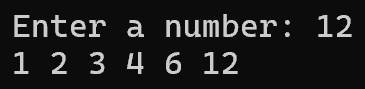
\includegraphics[height = .35in]{./imgs/factors1.PNG} \hfill  
		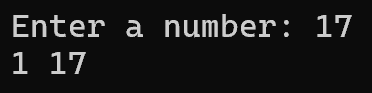
\includegraphics[height = .35in]{./imgs/factors2.PNG} \hfill  
		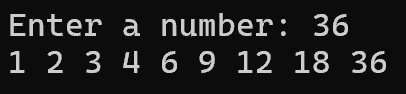
\includegraphics[height = .35in]{./imgs/factors3.PNG} \hfill \


%new_question
%%%%%%%%%%%%%%%%%%%%%
	% Problem 11
	% Difficulty: 1
%%%%%%%%%%%%%%%%%%%%%
	\item  
		%https://edabit.com/challenge/aqDGJxTYCx7XWyPKc
		Write a program that asks the user for an integer.  Calculate (and then print) the 
		sum of all square numbers up to and including the user's number.

		For example, 
		\begin{itemize}
			\item if user\_number = 3, the result should be 14 since $1^2 + 2^2 + 3^2 = 14$.
			\item if user\_number = 8, the result should be $1^2+2^2+3^2+4^2+5^2+6^2+7^2+8^2=204$.
		\end{itemize}

%end_of_questions


%standard 4.2

%start_of_questions


%new_question
%%%%%%%%%%%%%%%%%%%%%
	% Problem 4
	% Difficulty: 2
%%%%%%%%%%%%%%%%%%%%%
	\item   
		Write a program to create a word one letter at a time.  You should prompt the user to enter 
		a single letter one at a time until they type \textit{done}.  Once they type done, output 
		their newly created word.
		
		For example, \\ \ \hfill
		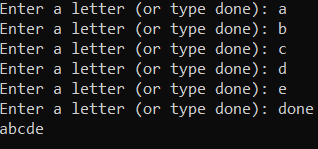
\includegraphics[width = 2.5in]{./imgs/lettersAbcde.PNG} \hfill  
		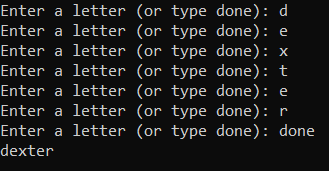
\includegraphics[width = 2.5in]{./imgs/lettersDexter.PNG} \hfill \


%new_question
%%%%%%%%%%%%%%%%%%%%%
	% Problem 6
	% Difficulty: 2
%%%%%%%%%%%%%%%%%%%%%
	\item  
		Write a program that repeatedly asks the user for integers until a negative integer is 
		given. \\ The program should keep track of the sum of the numbers and print the sum at the 
		end \\(not including the negative number).

		For example, \\ \ \hfill
		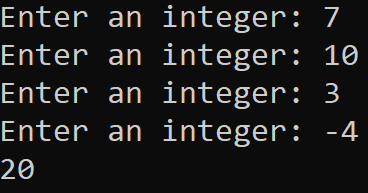
\includegraphics[width = 2.in]{./imgs/AddCalc2.PNG} \hfill  
		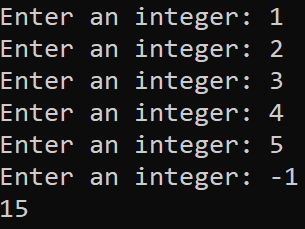
\includegraphics[width = 2.in]{./imgs/AddCalc1.PNG} \hfill \


%new_question
%%%%%%%%%%%%%%%%%%%%%
	% Problem 7
	% Difficulty: 2
%%%%%%%%%%%%%%%%%%%%%
	\item  
		Given a positive integer $n$, the following rules will always create a sequence that 
		ends with 1, called Hailstone Sequence:
		\begin{enumerate}
			\item If $n$ is even, divide by 2
			\item If $n$ is odd, multiply by 3 and add 1 (i.e. $3n+1$)
			\item Continue until $n$ is 1
		\end{enumerate}
		Write a program that prints the hailstone sequence starting at $n=25$.


%new_question
%%%%%%%%%%%%%%%%%%%%%
	% Problem 10
	% Difficulty: 2
%%%%%%%%%%%%%%%%%%%%%
	\item  
		%https://edabit.com/challenge/ksZrMdraPqHjvbaE6
		Write a program that repeatedly asks the user for integers until a negative integer is 
		given.\\  Report back the largest \textbf{even} number the user entered 
		(not including the negative number).  \\
		If the user didn't enter any even numbers report back $-1$.

		For example, \\ \ \hfill
		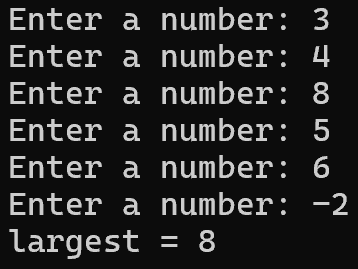
\includegraphics[height = 1.2in]{./imgs/largestEven1.PNG} \hfill  
		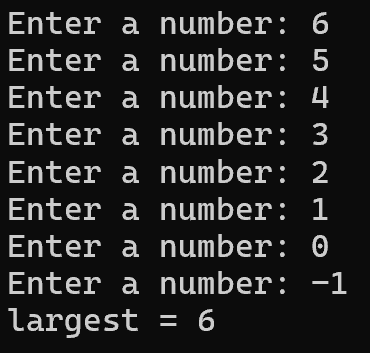
\includegraphics[height = 1.5in]{./imgs/largestEven2.PNG} \hfill  
		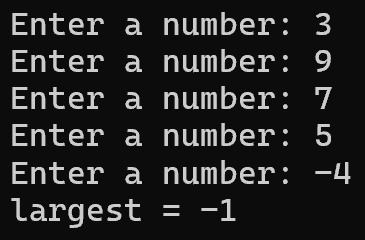
\includegraphics[height = 1.2in]{./imgs/largestEven3.PNG} \hfill \

%end_of_questions


%standard 4.3

%start_of_questions

%new_question
%%%%%%%%%%%%%%%%%%%%%
	% Problem 9
	% Difficulty: 3
%%%%%%%%%%%%%%%%%%%%%
	\item  
		%https://edabit.com/challenge/xR248CxGSsSrNK5Za
		You are the newest rug fashion designer on the scene, but you're running out of ideas. 
		Write a program that will help you design rugs.  The program should ask for a width, 
		a length, and pattern, and then create a rug consisting of that pattern and dimensions.

		For example, \\ \ \hfill
		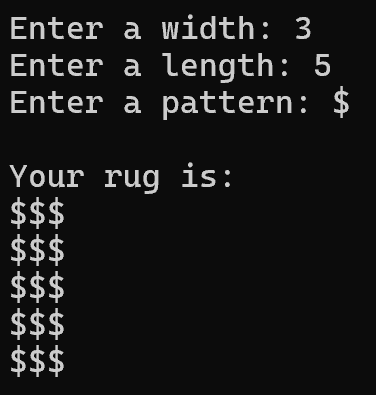
\includegraphics[width = 1.5in]{./imgs/rug1.PNG} \hfill  
		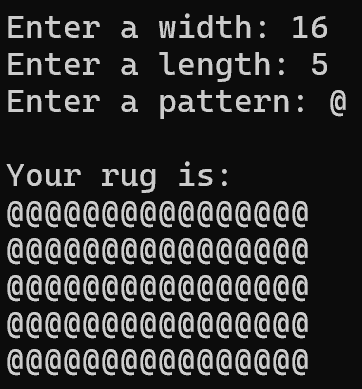
\includegraphics[width = 1.5in]{./imgs/rug2.PNG} \hfill \


%new_question
%%%%%%%%%%%%%%%%%%%%%
	% Problem 12
	% Difficulty: 3
%%%%%%%%%%%%%%%%%%%%%
	\item   
		Ask the user for two integer, and then build a multiplication table based on those numbers.

		For example, \\ \ \hfill
		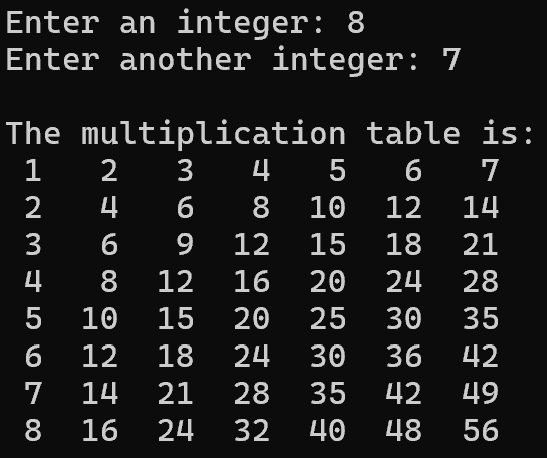
\includegraphics[height = 1.5in]{./imgs/mult_table1.PNG} \hfill  
		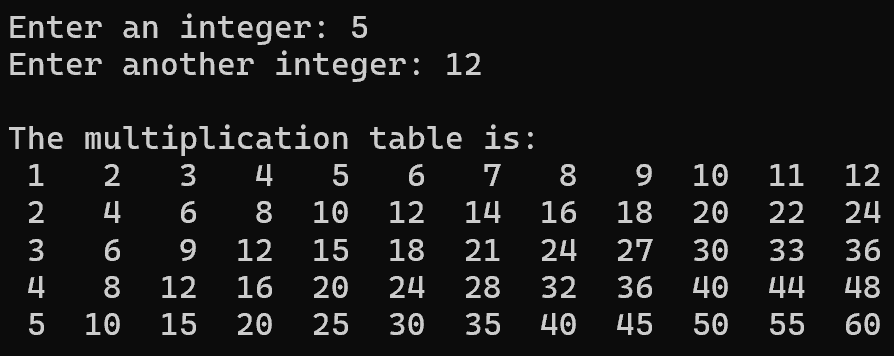
\includegraphics[height = 1.2in]{./imgs/mult_table2.PNG} \hfill  \


%new_question
%%%%%%%%%%%%%%%%%%%%%
	% Problem 13
	% Difficulty: 3
%%%%%%%%%%%%%%%%%%%%%
	\item  
		Ask the user for an integer height, and then build a triangle of asterisks (*) 
		with that height.

		For example, \\ \ \hfill
		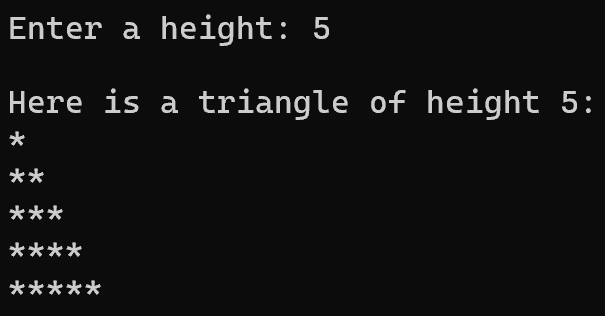
\includegraphics[height = 1.2in]{./imgs/triangle1.PNG} \hfill  
		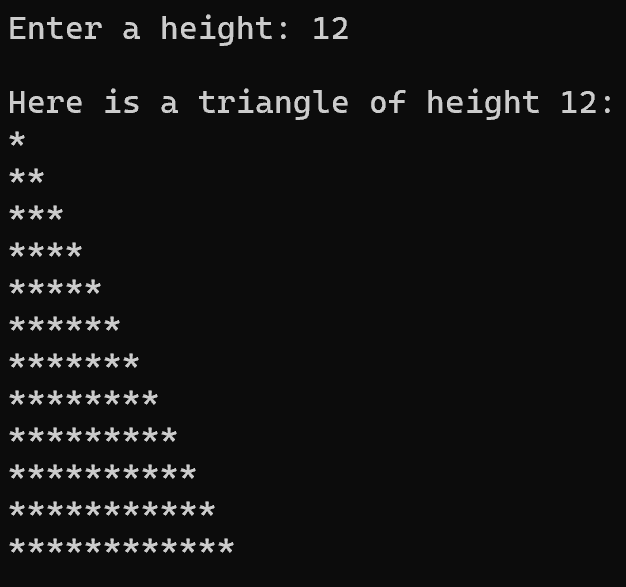
\includegraphics[height = 1.4in]{./imgs/triangle2.PNG} \hfill  \

%end_of_questions






%\item Write a program that will convert some amount of pennies into the fewest amount of dollars and coins possible.  For example, 75 pennies is 3 quarters.  86 pennies is 3 quarters, 1 dime, and 1 penny.  130 pennies is 1 dollar, 1 quarter and 1 nickel.  Let the user pick the number of pennies.  You may assume the largest input is 499 pennies.\\
%Hint: the way to do this is to always substitute for the largest denomination if available.  For example, if there is at least 100 pennies substitute for a dollar before quarters.

\end{enumerate}
\end{document}



%new_question
%%%%%%%%%%%%%%%%%%%%%
	% Problem 1
	% Difficulty: 1
%%%%%%%%%%%%%%%%%%%%%
	%paper-based
	\item 	
		In mathematics, the factorial of a non-negative integer n, denoted n\!, is the product of all positive
		integers less than or equal to n. See the table to the right for examples. Function $Fact$ that returns
		the factorial of a given non-negative integer.
		\begin{center}
		    \begin{minipage}{.4\textwidth}
		        \begin{tabular}{c|l|c}
		            \textbf{\( n \)} & \textbf{Product} & \textbf{\( n! \)} \\ \hline
		            0 & 1 & 1 \\
		            1 & 1 & 1 \\
		            2 & 2 $\times$ 1 & 2 \\
		            3 & 3 $\times$ 2 $\times$ 1 & 6 \\
		            4 & 4 $\times$ 3 $\times$ 2 $\times$ 1 & 24 \\
		            5 & 5 $\times$ 4 $\times$ 3 $\times$ 2 $\times$ 1 & 120 \\
		            6 & 6 $\times$ 5 $\times$ 4 $\times$ 3 $\times$ 2 $\times$ 1 & 720 \\
		        \end{tabular}
		    \end{minipage}
		\end{center}


\question[5]
	Write a program to create a word one letter at a time. You should prompt the user to enter a single letter 
	one at a time until they type done.  
	Once they type done, output their newly created word. See examples below.
	

	\begin{figure}[h]
	\centering
		\begin{minipage}{.5\textwidth}
		\centering
			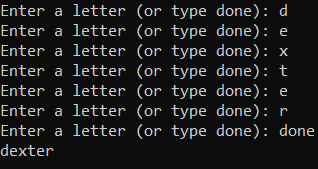
\includegraphics[height=2.5in]{./imgs/lettersDexter.png}
			\captionof*{figure}{Example 1}
		\end{minipage}%
			%
		\begin{minipage}{.5\textwidth}
		\centering
			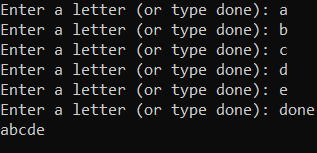
\includegraphics[height=2.5in]{./imgs/lettersAbcde.png}
			\captionof*{figure}{Example 2}
		\end{minipage}
	\end{figure}


%https://edabit.com/challenge/egMp3GWyN8TPptbZA
